\subsection{Pharos/TCRD target illumination: how druggable is the gated surfaceome?}
\label{sec:pharos}
DrugCentral (2021 snapshot) and Open Targets gave small-molecule- and
tractability-centric views; Pharos (TCRD, Illuminating the Druggable Genome)
assigns each human protein a Target Development Level (TDL: Tclin = target of
an approved drug with mechanism, including biologics; Tchem = potent
small-molecule ligands; Tbio = biology known, no ligands; Tdark = effectively
unstudied) plus a TIN-X novelty score. We queried the Pharos GraphQL API for
all @NGENES@ study genes (@NOK@ resolved to a target record; unresolved cases
carried forward as no-record) plus an EGFR sentinel.

\paragraph{Calibration gate.} Pre-registered gates PASSED: (G1) all four CAR-T
reference targets are Tclin (observed @GATEONE@); (G2) coverage @NOK@/@NGENES@
resolved records; (G3) at least three of four essential-gene controls are not
Tclin, confirming housekeeping is undrugged in the resource (observed
@GATETHREE@); (G4) the EGFR sentinel is Tclin in both Pharos and DrugCentral
(observed @GATEFOUR@).

\paragraph{Illumination of gated versus background.} Tclin fraction is
@TCLING@/@NG@ gated versus @TCLINB@/@NB@ background (Fisher odds ratio
@ORH1@, $p=@PH1@$). Full TDL mix gated: @MIXG@; background: @MIXB@. @H1VERDICT@
Median TIN-X novelty is @NOVG@ (gated) versus @NOVB@ (background)
(Mann--Whitney $p=@PH2@$; larger novelty means less studied). @H2VERDICT@
Median approved-drug count is @DRUGG@ versus @DRUGB@ ($p=@PH3A@$) and median
ligand count @LIGG@ versus @LIGB@ ($p=@PH3B@$).

\paragraph{Cross-source Tclin concordance.} Across @NCONC@ genes present in
both resources, Pharos and the 2021 DrugCentral snapshot agree on Tclin status
for @AGREEPCT@\% (Cohen's $\kappa=@KAPPA@$). Discordant genes (@NDISC@):
@DISCLIST@. @H4VERDICT@

\paragraph{AND-gate antigens.} @ANTIGENBLOCK@

\begin{figure}[t]
\centering
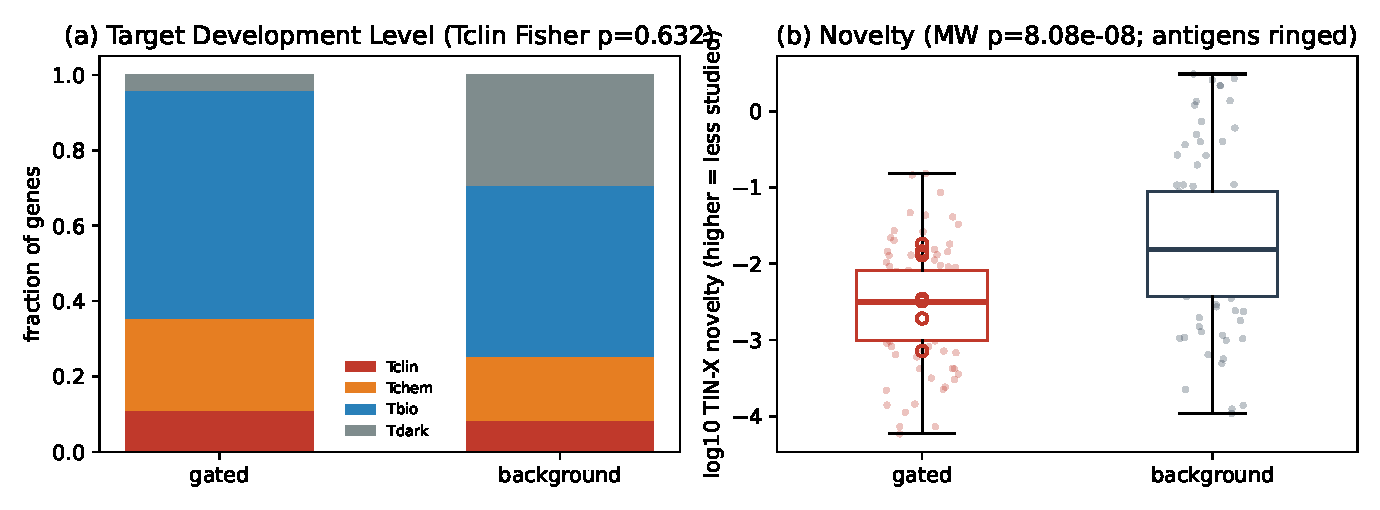
\includegraphics[width=\linewidth]{pharos_fig.pdf}
\caption{Pharos illumination audit. (a) Target Development Level mix for
gated versus background genes. (b) TIN-X novelty distribution (log scale;
higher = less studied), with the seven AND-gate antigens ringed.}
\label{fig:pharos}
\end{figure}
